% Copyright (c)  2005-2010 EDF-EADS-PHIMECA.
% Permission is granted to copy, distribute and/or modify this document
% under the terms of the GNU Free Documentation License, Version 1.2
% or any later version published by the Free Software Foundation;
% with no Invariant Sections, no Front-Cover Texts, and no Back-Cover
% Texts.  A copy of the license is included in the section entitled "GNU
% Free Documentation License".
\renewcommand{\filename}{docUC_RespSurface_PolyChaosDrawings.tex}
\renewcommand{\filetitle}{UC : Draw some usefull graphs associated to a polynomial chaos algorithm : polynomial graphs, comparison graph between numerical samples from the model and the meta-model, ...}

% \HeaderNNIILevel
% \HeaderIILevel
\HeaderIIILevel




The objective of this UC is to provide some graphs usefull after the launch of a polynomial chaos algorithm, as, for example :
\begin{itemize}
\item Graph 1 : the drawings of some members of the 1D polynomial family,
\item Graph 2 : the cloud of points making the comparison between the model values and the meta model ones : if the adequation is perfect, points must be on the first diagonal.
\end{itemize}


Details on response surface approximations may be found in the Reference Guide (\href{OpenTURNS_ReferenceGuide.pdf}{see files Reference Guide - Step Res. Surf. -- Functional Chaos Expansion and -- Polynomial Chaos Expansion}).\\

Details on each object may be found in the User Manual  (\href{OpenTURNS_UserManual_TUI.pdf}{see User Manual - Non Parametric Response Surface by Functional Chaos Expansion}).\\


The Use Case takes the example of the Jacobi family.\\

\requirements{
  \begin{description}
  \item[$\bullet$] the distribution of the input random vector : {\itshape inputDistribution}
  \item[type:]  a Distribution
  \item[$\bullet$] the limit state function : {\itshape limitStateFunction}
  \item[type:]   a NumericalMathFunction
  \item[$\bullet$] the meta model : {\itshape metaModel}
  \item[type:] a NumericalMathFunction
  \end{description}
}
{
  \begin{description}
  \item[$\bullet$] graphs described above : {\itshape graphJacobi, graphCloud}
  \item[type:] Graph
  \end{description}
}


\textspace\\
Python  script for this UseCase :


\begin{lstlisting}
  #################################################
  # GRAPH 1 : drawings of the 5-th first members of
  # the Jacobi family

  # Create the Jacobi polynomials family
  alpha = 0.5
  beta = 1.5
  jacobiFamily = JacobiFactory(alpha, beta)

  # Fix the degree max of the polynomials
  # which will be drawn
  degreeMax = 5

  # Load all the valid colors
  colorList = Drawable.GetValidColors()

  # Create a fine title
  titleJacobi = "Jacobi(" + str(alpha) + ", " + str(beta) + ") polynomials"

  # Create an empty graph which will be fullfilled
  # with curves
  graphJacobi = Graph(titleJacobi, "z", "polynomial values", True, "topright")

  # Fix the number of points for the graph
  pointNumber = 101

  # Bounds of the graph
  xMinJacobi = -1
  xMaxJacobi = 1

  # Get the curves
  for i in range(degreeMax) :
  graphJacobi_temp = jacobiFamily.build(i).draw(xMinJacobi, xMaxJacobi, pointNumber)
  graphJacobi_temp_draw = graphJacobi_temp.getDrawable(0)
  legend = "degree " + str(i)
  graphJacobi_temp_draw.setLegendName(legend)
  graphJacobi_temp_draw.setColor(colorList[i])
  graphJacobi.addDrawable(graphJacobi_temp_draw)

  # In order to see the graphs without creating the files .EPS, .PNG and .FIG
  Show(graphJacobi)

  # Create the files .EPS, .PNG and .FIG
  graphJacobi.draw("PCE_JacobiPolynomials")

  # Visualize the file .PNG wihthin the TUI
  ViewImage(graphJacobi.getBitmap())


  #####################################################
  # GRAPH 2 : points cloud between model and meta model

  # Generate a NumericalSample of the input random vector
  sizeX = 500
  Xsample = inputDistribution.getNumericalSample(sizeX)

  # Evaluate the model on the sample
  modelSample = limitStateFunction(Xsample)

  # Evaluate the meta model on the sample
  metaModelSample = metaModel(Xsample)

  # Create the numerical sample of points (Y, Y_tilde)
  sampleMixed = NumericalSample(sizeX,2)
  for i in range(sizeX) :
  sampleMixed[i][0] = modelSample[i][0]
  sampleMixed[i][1] = metaModelSample[i][0]

  # Create a fine title
  legend = str(sizeX) + " realizations"

  # Create the cloud
  comparisonCloud = Cloud(sampleMixed, "blue", "fsquare", legend)

  # Put it within a graph structure
  graphCloud = Graph("Polynomial chaos expansion", "model", "meta model", True, "topleft")

  # Fulfill the graph with the cloud
  graphCloud.addDrawable(comparisonCloud)

  # In order to see the graphs without creating the files .EPS, .PNG and .FIG
  Show(graphCloud)

  # Create the files .EPS, .PNG and .FIG
  graphCloud.draw("PCE_comparisonModels")

  # Visualize the file .PNG wihthin the TUI
  ViewImage(graphCloud.getBitmap())
\end{lstlisting}

\vspace*{0.1cm}

The example illustrated here below is the beam example described in Eq. (\ref{equatPoutre}), where :
\begin{itemize}
\item $E$ follows the Beta($r = 0.9$, $t = 3.2$, $a = 2.8e7$, $b = 4.9e7$) distribution,
\item $F$ follows the Gamma($k = 3e5$, $\lambda = 9e3$, $\gamma = 1.5e4$)  distribution,
\item $L$ follows the Uniform($a = 250$, $b=260$) distribution,
\item $I$ follows the Beta($r = 2.5$, $t = 4.0$, $a = 3.1e2$, $b = 4.5e2$) distribution,
\item the four components are independent.
\end{itemize}

We took the following 1D polynomial families, which parameters have been determined in order to be adapted to the marginal distributions of the input random vector :
\begin{itemize}
\item $E$ : Jacobi($\alpha = 1.3$, $\beta = -0.1$),
\item $F$ : Laguerre($k = 1.78$),
\item $L$ : Legendre,
\item $I$ : Jacobi($\alpha = 0.5$, $\beta = 1.5$).
\end{itemize}

The truncature strategy of the multivariate orthonormal basis is the Cleaning Strategy where we considered within the $500$ first terms of the multivariate basis, among the 50 most significant ones, those which contribution wre significant (which means superior to $10^{-4}$).\\

The evaluation strategy of the approximation coefficients is the least square strategy based on a experiment plane determined with the Monte Carlo sampling technique of size 100.\\

Figures (\ref{PCE_E}) to (\ref{ModelsComparison}) draw the graphs mentioned above.




\begin{figure}[H]
  \begin{minipage}{9cm}
    \begin{center}
      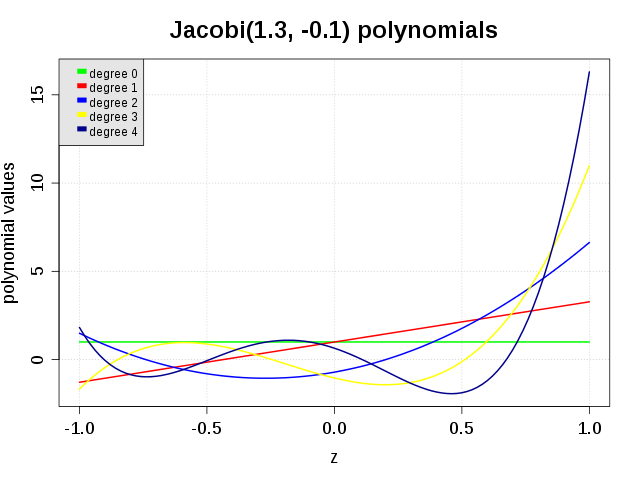
\includegraphics[width=7cm]{PCE_JacobiPolynomials_VariableE.png}
      \caption{The 5-th first polynomials of the Jacobi family associated to the variable E.}
      \label{PCE_E}
    \end{center}
  \end{minipage}
  \hfill
  \begin{minipage}{9cm}
    \begin{center}
      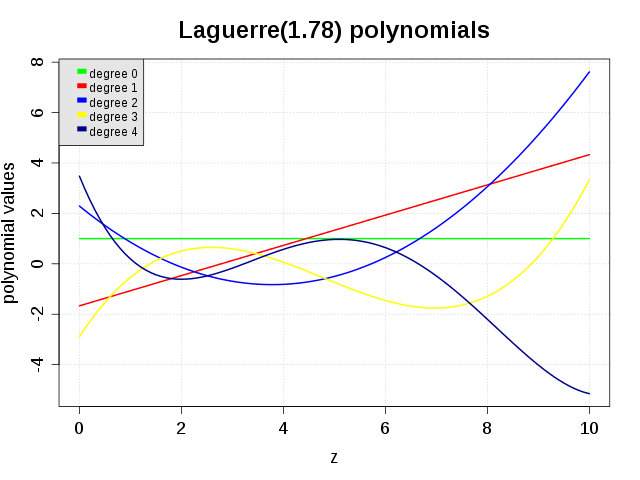
\includegraphics[width=7cm]{PCE_LaguerrePolynomials_VariableF.png}
      \caption{The 5-th first polynomials of the Laguerre family associated to the variable F.}
      \label{PCE_F}
    \end{center}
  \end{minipage}
\end{figure}

\begin{figure}[H]
  \begin{minipage}{9cm}
    \begin{center}
      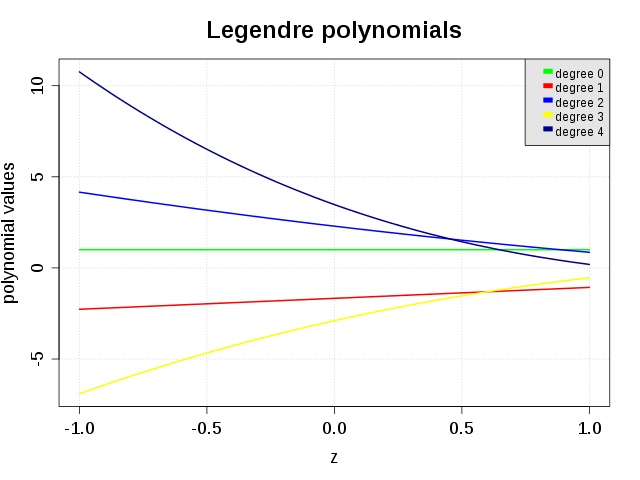
\includegraphics[width=7cm]{PCE_LegendrePolynomials_VariableL.png}
      \caption{The 5-th first polynomials of the Legendre associated to the variable I.}
      \label{PCE_L}
    \end{center}
  \end{minipage}
  \hfill
  \begin{minipage}{9cm}
    \begin{center}
      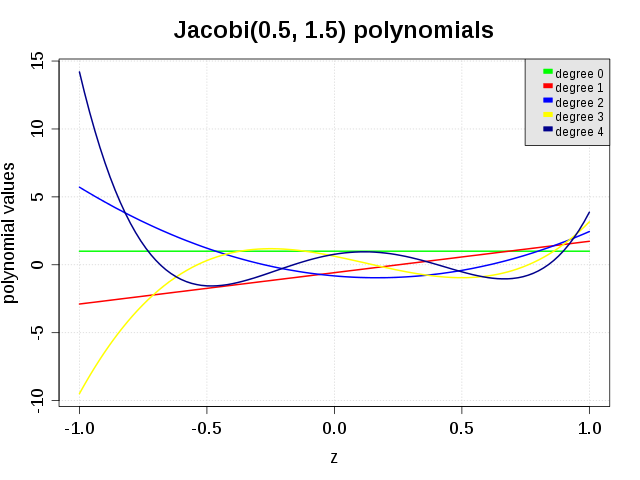
\includegraphics[width=7cm]{PCE_JacobiPolynomials_VariableI.png}
      \caption{he 5-th first polynomials of the Jacobi family associated to the variable I.}
      \label{PCE_I}
    \end{center}
  \end{minipage}
\end{figure}




\begin{figure}[H]
  \begin{center}
    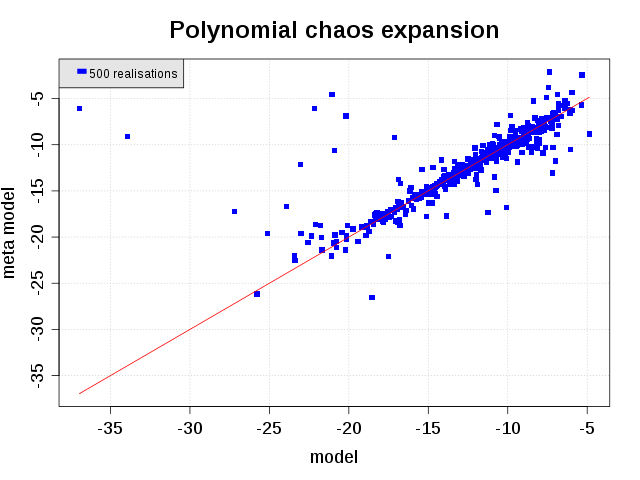
\includegraphics[width=7cm]{PCE_comparisonModels.png}
    \caption{Comparison of values from the model and the polynomial chaos meta model.}
    \label{ModelsComparison}
  \end{center}
\end{figure}


Figures (\ref{PCE_Kraw}) to (\ref{PCE_Char}) draw the  5-th first polynomials of the Krawtchouk and Charlier  family respectively associated to the $Binomial(N=5,p=0.6)$ and $Poisson(0.6)$ distributions.



\begin{figure}[H]
  \begin{minipage}{9cm}
    \begin{center}
      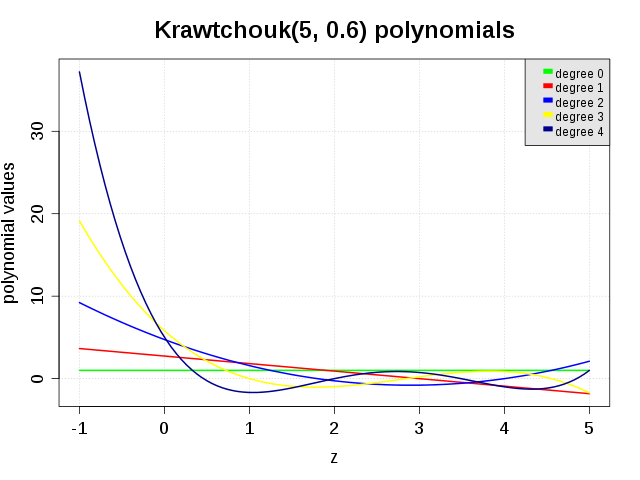
\includegraphics[width=7cm]{PCE_KrawtchoukPolynomials.png}
      \caption{The 5-th first polynomials of the Krawtchouk associated to the  $Binomial(N=5,p=0.6)$ measure.}
      \label{PCE_Kraw}
    \end{center}
  \end{minipage}
  \hfill
  \begin{minipage}{9cm}
    \begin{center}
      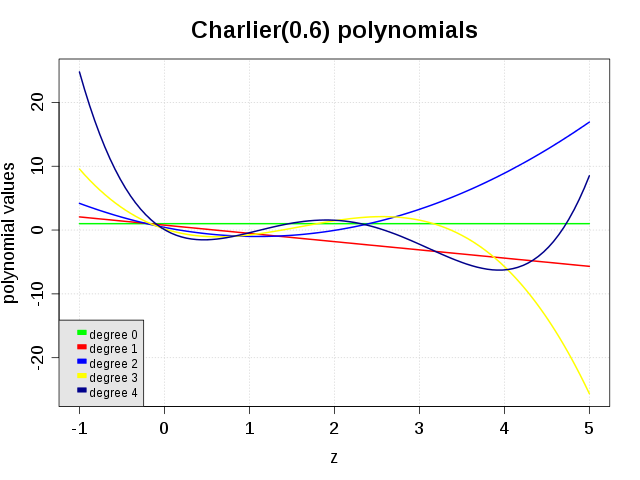
\includegraphics[width=7cm]{PCE_CharlierPolynomials.png}
      \caption{The 5-th first polynomials of the Charlier  family associated to the $Poisson(0.6)$ measure.}
      \label{PCE_Char}
    \end{center}
  \end{minipage}
\end{figure}

